\documentclass[a4paper,11pt,oneside]{article}

\usepackage[latin1,utf8]{inputenc}
\usepackage[english, english]{babel}
\usepackage{amsmath, amsfonts, amssymb, amsthm}
\usepackage{graphicx}
\usepackage[hmargin=25mm,vmargin=25mm]{geometry}
\usepackage{hyperref} %per i collegamenti
\usepackage{listings}
\usepackage[small,bf]{caption}
\usepackage{subcaption}
\usepackage{graphicx}
\usepackage{pgf}
\usepackage{tikz}
\usepackage{pgfplots}
\usepackage{pgfplotstable}
\usepackage{amssymb}

\pgfplotsset{
	every axis/.append style={thick,tick style={semithick}},
	legend style={font=\footnotesize,rounded corners=2pt},
	tick label style={font=\small},
	label style={font=\small}
}


\DeclareMathOperator{\score}{score}


\hypersetup{
    colorlinks=true,       % false: boxed links; true: colored links
    linkcolor=red,          % color of internal links
    citecolor=green,        % color of links to bibliography
    filecolor=magenta,      % color of file links
    urlcolor=cyan           % color of external links
}

\title{\textbf{{\huge Information Retrieval Final project}}}
\author{Emilio Del Tessandoro 412888, Chiara Marcheschi 303756}
\begin{document}
\maketitle


\section{Introduction}
\label{sec:intro}
The purpose of this project is to extract semantic information from a set of tweets: tweets are short texts or phrases written by the Twitter users. In this work we have to deal both with semi-structured and unstructured data, since the informations we manipulate are stored in JSON format, but the tweet text is of course a non structured kind of data.
%In addition to the problem of manipulating unstructured data, an other problem, that we must considered, is that of retrieve the information from the huge amount of data.
The size of the data is very big and, for storing tweets of some hundreds of thousands of users are necessary many GBs of space. Moreover, given the nature of the data, it is very difficult to make analysis that are different from the syntactical one.

For these reasons, before using the dataset for obtaining semantic information, it's necessary to process the data several times, using filters and clustering tools. Our purposes are many and range over a wide variety of fields:

\begin{enumerate}
 \item Study the graph of politicians and their followers (section \ref{sec:graph}). Could be very important to discover connecting links between a politician and his followers, for building the twitter social connection net.
 \item Study the topics of the tweet text. For this purpose we used tools of TAGME (section \ref{sec:tagme}).
 \item Study the semantic information hidden in the hashtags (section \ref{sec:hashtags}). Often an hashtag can be considered the topic-tag of the tweet.
 \item Discover the ``sentiment'' hidden in the tweet text (section \ref{sec:sentiment}), performing what is called sentiment analysis. In particular we propose to distinguish tweets about politics from others, for operating the analysis only on the first set.
 \item Build a global view of the political sentiment based on this tweets semantic study (section \ref{sec:exitpoll}).
\end{enumerate}

Twitter collects thoughts from all over the world and it's our task to translate the tweets in useful information.
In the next sections we will address the different topics, tackled by us.

\subsection{Dataset}
We had at our disposal two datasets. The first one given is described in the slides of the project and consists of these files:
\begin{enumerate}
\item \texttt{TweetTwitter-20110912\_160840.userinfo} (the users file), containing \emph{informations} about 170000 users that are followers of 7 given italian politicians  (in JSON format).
\item \texttt{TweetTwitter-20110912\_160840.tweet} (the tweets file), containing \emph{tweets} of 170000 users that are followers of 7 given italian politicians  (in JSON format).
\item \texttt{TweetTwitter-20110912\_160840.graph} (the graph file), containing the \emph{associations} between politicians and followers (that is the users which follow a given politician).
%In realta questi tre sono stati generati da paurullan e dai 3 terroni!!
%\item ``TweetTwitter-20110912\_160840.text'' Teewts Text, containing the associations idTweet-textTweet.
%\item ``TweetTwitter-20110912\_160840.list'' containing a number of tweets from the users.
%\item ``TweetTwitter-20110912\_160840.info'' and ``TweetTwitter-20110912\_160840.fc'' Info dataset.
\end{enumerate}

The other dataset has been downloaded by the group composed by Daniele De Sensi, Andrea Cicalese and Francesco Piccinno (so refer to their report for other details), and we used in particular the tweets of the users, not the politicians.
These users are the followers of 13 politicians (the 7 of the initial dataset and other 6) that wrote at least one tweet every 10 days, on average. Of these users they took the whole timeline, for a total of of 21.6 millions tweets.

\begin{table}[h]
\begin{center}
	\begin{tabular}{l | c | c | c | c}
	%\hline
	& total users & politicians & total tweets & size\\ \hline
	first dataset & 173K & 7 & about 884K & 79MiB\\ %\hline
	second dataset & about 20K & 13 & 21.6M & 2.2GiB
	\end{tabular}
\end{center}
\caption{A quick overview of the two datasets sizes and characteristics.}
\end{table}




\section{The users graph}
\label{sec:graph}
Here we wanted analyse the structure of the users graph. In particular we are interested in finding the users that follows more than one politician. For this purpose we ``inverted'' the graph file given in the first data set: instead of having for every politician the list of users that are him followers, we create, for every user, the list of politicians followed by that user.
So we have a list of pairs \textit{(user, list of politicians)}, that can be easily sorted on the politicians list length in order to view the users that follows $x$ politicians. We obtained the following results on the first data set:

\begin{table}[h]
\begin{center}
	\begin{tabular}{l | r}
	%\hline
	Following 1 politician: & 127037\\ %\hline
	Following 2 politicians: & 30667\\ %\hline
	Following 3 politicians: & 12731\\ %\hline
	Following 4 politicians: & 2101\\ %\hline
	Following 5 politicians: & 400\\ %\hline
	Following 6 politicians: & 99\\ %\hline
	Following 7 politicians: & 8\\ \hline
	Total:	 & 173043 \\
	& (+7 politicians)\\ %\hline
	\end{tabular}
\end{center}
\caption{Statistics of the users of the first dataset. Remember that the total number of politicians is 7. We curiously found that the politician 14078646 (Idvstaff) follows the politician 19067940 (beppe\_grillo).}
\end{table}

This part, and also others, has been developed in python (see script \texttt{graph.py}).

\subsection{Further work about the graph}
The informations we have at our disposal are limited to a set of seven politicians and their followers. The directed edges of this graph are important, because they represent a contact between users. Most connected parts of the graph correspond to ``communities'' of users. We can exploit the structure of this graph in order to have a score similar to PageRank. This score can be used in different cases; the basic idea is that a term is more relevant if it appears in the tweets of an important user (in terms of this score).

Moreover this kind of reasoning can be extended if we consider not only the direct connections\footnote{Connection given by the fact that an user follows another.}, but also connections given by conversations (retweets and replies, see also \ref{fig:twitterGraph}) and citations (tweets containing \emph{``@user''}).
These informations can be used to build new levels of connection between users or to weight the existing ones.

\begin{figure}[htbp]
  \begin{subfigure}[h]{\textwidth}
    \centering
    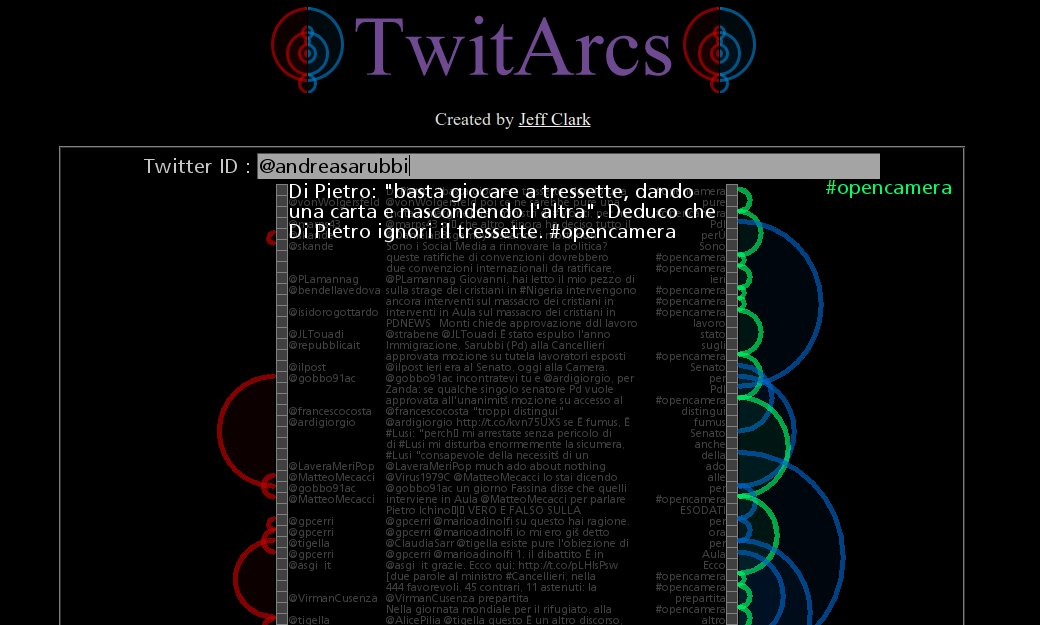
\includegraphics[width=0.8\textwidth]{./image/twitArcs.jpg}
    \caption{Example of twitArcs-use (arcs are drawn on the left connecting people that are repeated and on the right for common repeated terms), result of Jeff Clark's work \cite{clark3}.}
    \label{fig:twitArcs}
  \end{subfigure}
  \hspace{8mm}
  \begin{subfigure}[h]{\textwidth}
    \centering
    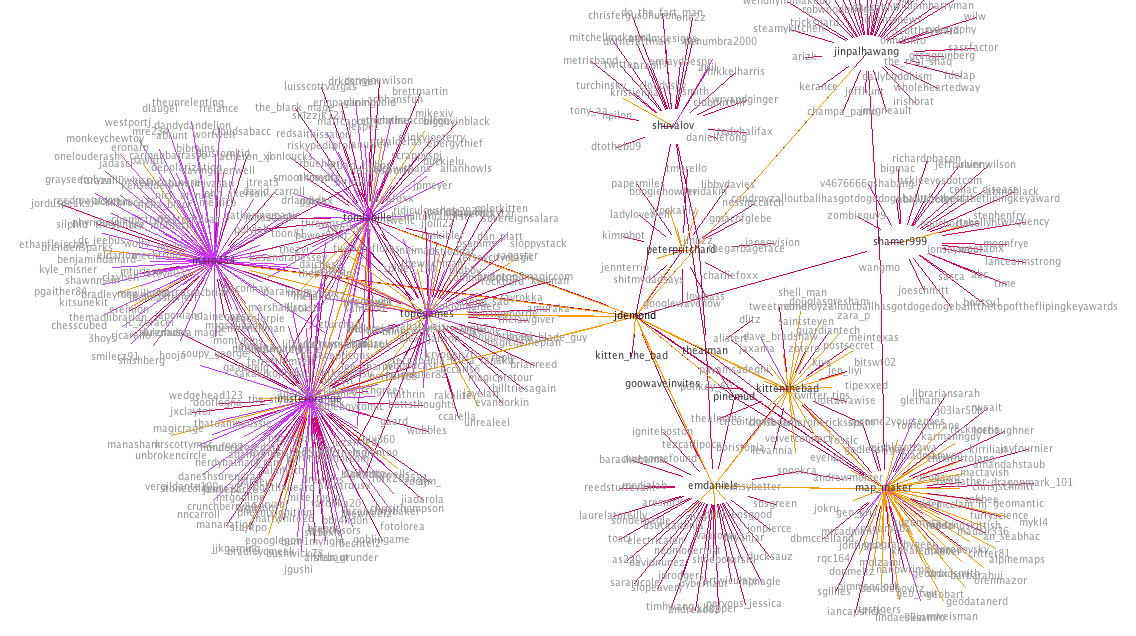
\includegraphics[width=01\textwidth]{./image/jdemondGraph.png}
    \caption{Example of a twitterGraph (jdemond's graph: @jdemond's Twitter Conversation Network), result of Cate Huston's work \cite{huston}.}
    \label{fig:twitterGraph}
   \end{subfigure}
   \caption{Examples of connection-graphs build over users-connections.}
  \label{fig:graph}
\end{figure}

\subsection{The graph of the terms}
As just introduced Twitter makes possible to build conversations among users. The metadata associated to a tweet contain the necessary informations to build these conversations, that can be then analysed and decomposed into words.

The way of utilization, the frequency and the association of words, hashtags, citations, links, inside the tweets, can give sufficient informations for developing graphs also on the terms (see figure \ref{fig:tweetSpectrum}). If these informations, about the words used by the community, are stored and organized chronologically, we can observe the different terms usage during time (figure \ref{fig:twitterStreamGraphs}).

This is outside our goals, also for the lack of informations in the datasets at our disposal.

\begin{figure}[htbp]
  \begin{subfigure}[h]{\textwidth}
    \centering
    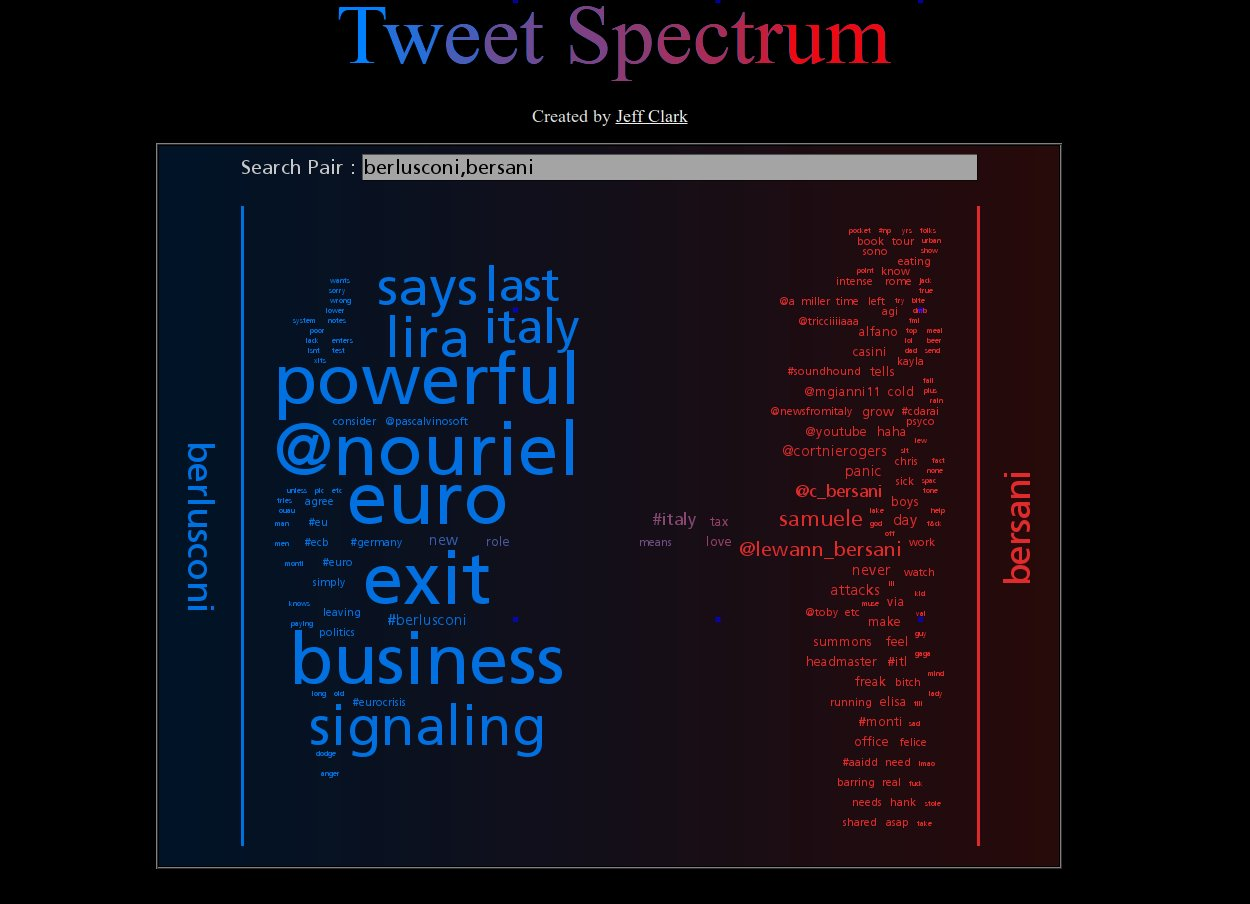
\includegraphics[width=0.76\textwidth]{./image/tweetSpectrum.jpg}
    \caption{Example of tweetSpectrum-use (relatived-terms about a pair of words), result of Jeff Clark's work \cite{clark2}.}
    \label{fig:tweetSpectrum}
  \end{subfigure}
  \hspace{8mm}
  \begin{subfigure}[h]{\textwidth}
    \centering
    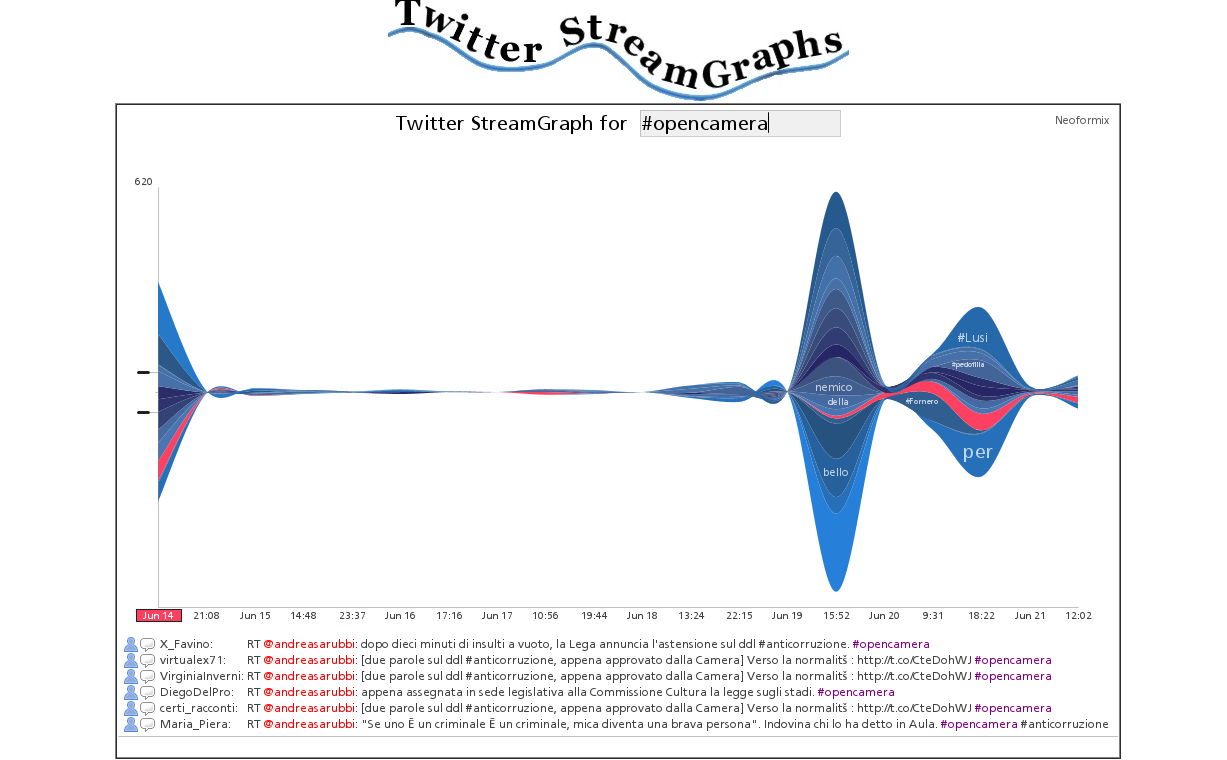
\includegraphics[width=0.76\textwidth]{./image/twitterStreamGraphs.png}
    \caption{Example of twitterStreamGraphs-use (StreamGraph shows for the latest 1000 tweets which contain the search word), result of Jeff Clark's work \cite{clark1}.}
    \label{fig:twitterStreamGraphs}
   \end{subfigure}
   \caption{Examples of connection-graph build over word-connections.}
  \label{fig:wordsGraph}
\end{figure}


\section{Tweets annotation}
\label{sec:tagme}
We have used \href{http://tagme.di.unipi.it/}{TAGME} to annotate tweets, associating some topics to each tweets of the dataset. The topics is associated to the tweets only of the annotation has rho greater than a default threshold, with value 0.2.
The tweets, before being processed with TAGME, are cleaned by urls, quotes (so written \textit{@users}). This process is necessary for making tweets more similar to a sentence.
It could be useful to do analysis about tweets language, for rejecting those not supported by TAGME and indicating to it the language to using for the annotation.
We have done a simplification in the analysis, assuming that all tweets were written in Italian (only a small percentage of those uses a different language).
An additional preprocessing done above tweets, is the replacement of numeric character references in tweets (like in all web text, \textsl{\&\#N;}, where \textit{N} is a number) with its unicode character.


\section{Hashtags semantic}
\label{sec:hashtags}
In this part we used the tweets from the users of the second dataset, because it was bigger. We tried to use \href{http://tagme.di.unipi.it/}{TAGME} to give to hashtags a meaning, that is associating to each hashtag a list of topics that can be taken as its ``description''. We also wanted to rank these topics, for every tag.

We proceeded in the following steps:

\begin{enumerate}
\item Select only tweets that contains at least an hashtag. This has been done with a simple bash command. The tweets those use at least one hashtag are about 16\% of the total (about 3.4 millions over 21).
\item Filter only tweets that has at least one annotation. This has been done with the script \texttt{tweetsFilter.py}, which opens both the tweet file and the annotated one, discarding tweets with no annotation in the second file.
\item Collect for every user all the pairs $(h,a)$, where $h$ is an hashtag and $a$ an annotation. If for user $u$ exist such a pair, means that $u$ wrote some tweets where $h$ appear as hashtag, and these tweets are annotated with $a$. 
%What relation there is between an hashtag and an annotation, $(h,a)$? Intuitively how much near is the meaning of hashtag $h$ and that of annotation $a$.
We actually approximate the meaning of an hashtag with some kind of metrics based on the frequency of couple $(h,a)$ in the tweets of the user $u$, on its reliability ($\rho$ of annotations) and the number of users that use the hashtag $h$ with meaning $a$. We indicate this metrics with a weight $w(u,h,a)$ that can be computed using the factors just introduced.

A first approach can be to consider the number of times that the pair $(h,a)$ has been used by $u$. In this case:
\begin{equation}
w(u,h,a) = f(u,h,a) = \text{number of times user $u$ used association $(h,a)$}
\end{equation} 
A second approach could be to use the sum of the \textit{rho}s of the annotations we are talking about (instead of the raw tweet count). In this case we have instead:
\begin{equation}
w(u,h,a) = P(u,h,a) = \text{sum of $\rho$'s of annotations where $u$ used the association $(h,a)$}
\end{equation} 
For further details see the script \texttt{hashtagAnnotation.py}.
\item Merge all the informations produced above creating a unique score for association $(h,a)$, summing up the contributions of the various users. This has been done with the script \texttt{hashtagMerge.py}. Here the annotations are sorted by their importance, as explained in section \ref{sec:merge}.
\end{enumerate}

The last two points could have been realized in one single step, but for simplicity and further extensions we preferred to keep the two parts separated. The time (and I/O) complexity of the first two steps is linear in the number of tweets: it is necessary to keep only one tweet at the time in the internal memory. 
The other two steps instead require to build some kind of dictionary containing the associations between every user and its pairs $(h,a)$. This, with the datasets at our disposal, can be easily done in internal memory\footnote{We used the built-in python \texttt{dict}.} but, if the dataset is bigger we have to use I/O efficient data structures.

%Notice that as we built associations of the type $(h,a)$ (that is, for every  we can easily ``invert'' this if we want to manage $(a,h)$ pairs, as we done in section \ref{sec:tagger}.

\subsection{How the merge works}
\label{sec:merge}
One fundamental step in the previous procedure is how to merge together informations coming from different users into a single score. We assumed three possible score measures that are very simple to calculate and give a base for furter reasoning. They are, for a fixed pair $\langle h,a \rangle$, (hashtag, annotation):
\begin{enumerate}
\item the user count $u(h,a)$, that is simply the number of users that used the pair $<h,a>$ in at least one tweet, indifferently from the number of these tweets. Having a high $u(h,a)$ is an indication of the popularity of the pair $\langle h,a \rangle$: the hashtag $h$ is used by many users with meaning $a$.

\item the total number of tweets where the $\langle h,a \rangle$ pair is used, disregaring any information about the users (i.e. the previous indicator). We will indicate this number with $\mathcal{F}(h,a)$. This can be easily calculated if $w(u,h,a)$ simply represent the number of tweets written by $u$, where the pair $\langle h,a \rangle$ is used. In formulas:
\begin{equation}
\label{eqn:frequency}
\mathcal{F}(h,a) = \sum_{u} f(u,h,a)
\end{equation}
An $u(h,a)$ high means that the hashtag $h$ is used often with meaning $a$. On the other hand it can be the result of spamming of a single user.

\item the total sum of the \textit{rho}s if $w(u,h,a)$ is instead based on a $\rho$-weighting. This number will be indicated with $\mathcal{P}(h,a)$ in the following part.
\begin{equation}
\mathcal{P}(h,a) = \sum_{u} P(u,h,a)
\end{equation}
\end{enumerate}

It's clear that the last two measures are strongly related, and in general they are equal except for a constant factor. Also the first measure $u(h,a)$ is related to the second. In fact is possible to notice that:
\begin{equation}
\label{eqn:step}
u(h,a) = \sum_{u} \boldsymbol{1}_{(0,\infty)}\left( f(u,h,a) \right)
\end{equation}
Where $ \boldsymbol{1}_{(0,\infty)}(x) $ is the step function returning 1 only for values greather than 0. This clearly holds because if $ f(u,h,a) $ is greather than 0 means that user $u$ wrote at least one tweet where association $ (h,a) $ exists. The step function makes this contribution count as one.
The measure $\mathcal{F}(h,a)$ (equation \ref{eqn:frequency}) is similar but with a linear function in place of $\boldsymbol{1}_{(0,\infty)}(x)$.
Having in mind this consideration one can also observe that: %So how to combine these possibilities in a single score?

\begin{itemize}
\item $u(h,a)$ is important in the final score.
\item $\mathcal{F}(h,a)$ (or $\mathcal{P}(h,a)$) shouldn't be negligible. In other words the number of users that used association $(h,a)$ is clearly important, but there should be also some dependance, in the score, on how many times (or how often) a certain user used that association.
An high frequency of hashtag $h$ correspondes to a bigger importance of $h$ (with a given meaning $a$), it must appear in the score.
\end{itemize}

%The number of messages written by $u$ can be a factor to normalize $f(h,a)$ (or $P(h,a)$), in order to get a measure that is closer to $u(h,a)$. 
A possible idea is to use a different function in equation \ref{eqn:step} (something between a step function and a linear function) in order to get a measure that is closer to $ u(h,a) $ but increasing with $ \mathcal{F}(h,a) $. A good score measure can be:

\begin{equation}
\label{eqn:score}
\score (h,a) = \sum_{u} \log \left( 1 + w(u,h,a) \right) 
\end{equation}

Notice that if the logarithm in equation \ref{eqn:score} is in base 2 and the weights used are the number of tweets (so $w(u,h,a) = f(u,h,a)$), the result of this score is always between $u(h,a)$ and $\mathcal{F}(h,a)$.
In fact the argument of the logarithm will be one if there are no tweets for user $u$ containing the hashtag $h$ with meaning $a$, otherwise it will have always a value greater or equal to two, since $\mathcal{F}(h,a)$ (for user $u$) will be always greater or equal to one.

\begin{table}[h]
\centering{
\begin{tabular}{c | c | c | c}
%\hline
example of $f(u,h,a)$ weights for 20 users & $u(h,a)$ & $\score(h,a)$ & $\mathcal{F}(h,a)$\\
\hline
1,  1, 1, 1, 1, 1, 1, 1, 1, 1, 6, 1, 1, 1, 2, 1, 2, 1, 1, 2 & 20 & 24.15 & 29 \\
15, 1, 2, 1, 1, 1, 1, 1, 1, 1, 6, 1, 1, 1, 2, 1, 2, 1, 1, 2 & 20 & 27.15 & 43 \\
3,  4, 2, 3, 4, 4, 2, 1, 1, 1, 6, 1, 1, 1, 2, 1, 2, 1, 1, 2 & 20 & 30.70 & 43
\end{tabular}
}
\caption{An example of the 3 score measures. Notice how, in the last two cases $\score(h,a)$ increases while $\mathcal{F}(h,a)$ remain constant. The difference in the two cases is that in the second row we have a high spike in the number of messages by a certain user, while, in the third row, although the total number of tweets is the same, so the use of hashtag $h$ (with meaning $a$) is better-balanced among more users.}
\end{table}

%per allineamento immagini con testo ...
%\newpage

\subsection{Popularity vs Frequency}
Preceding observations about count of the score, suggest us to examine the distribution of hashtags over user-set and tweet-set. The results of this analysis will give us an index of the gooodness of the score count method (equation \ref{eqn:score}).
We plotted more graphs of hashtags sorted by frequency, trascribing the frequency (in red) and the number of users those using that hashtag (in green) (see figure \ref{fig:plotFrequency}).

%\begin{figure}[h]
%\centering
%\subfloat[][\emph{Sum of $\rho$ for each hashtag}.]
%{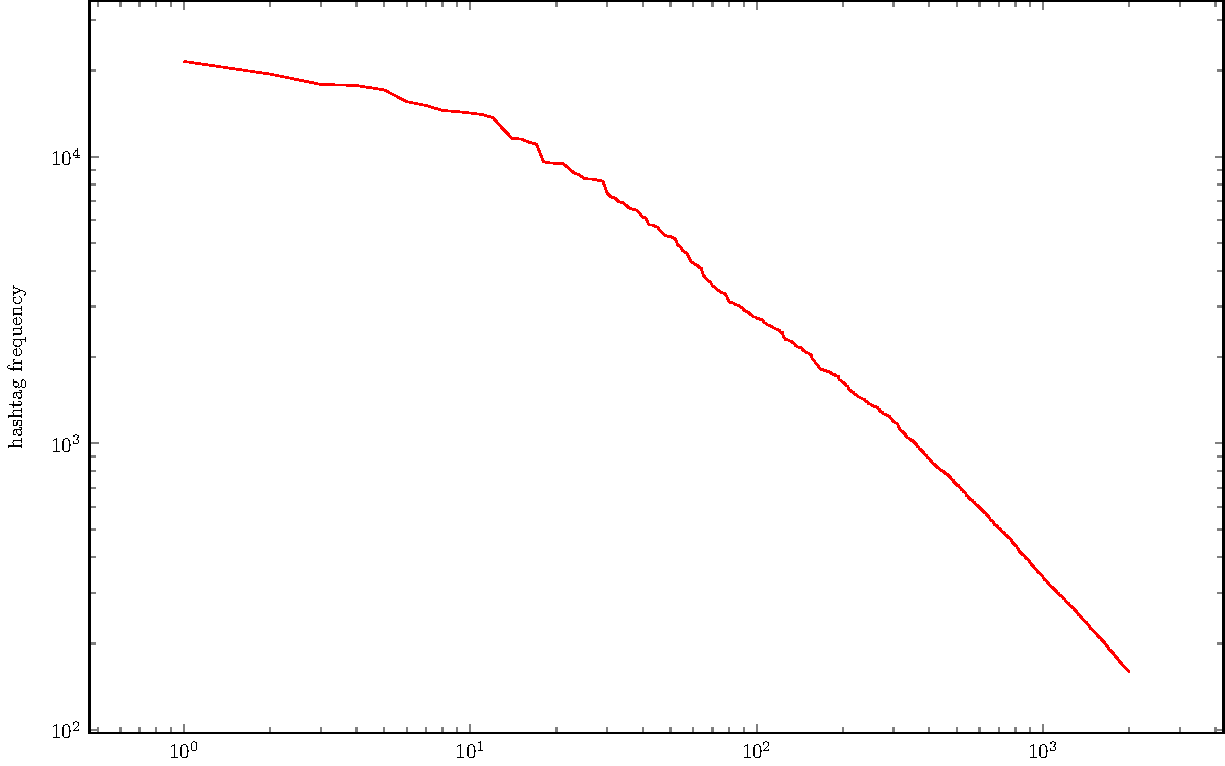
\includegraphics[width=.45\columnwidth]{./image/plotSumOfRhos.pdf}}\quad
%\subfloat[][\emph{$\score(h,a)$ for each hashtag}.]
%{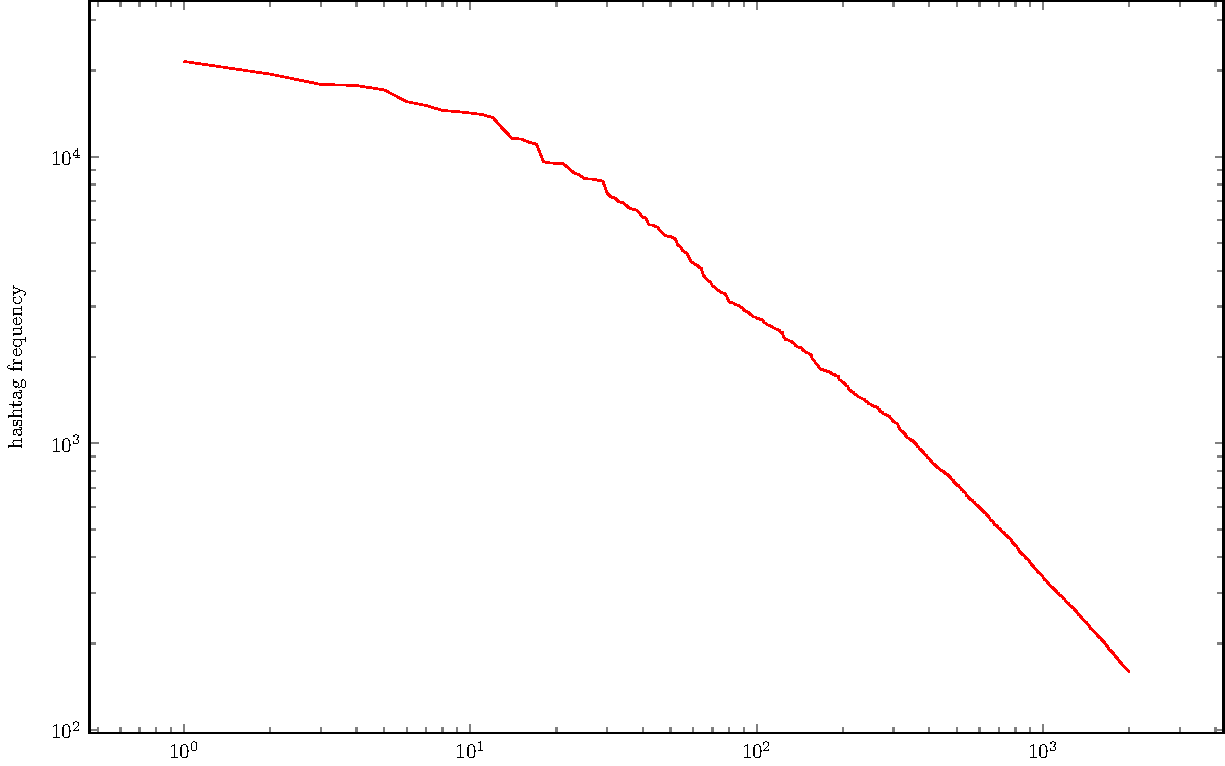
\includegraphics[width=.45\columnwidth]{./image/plotSumOfRhos.pdf}}
%\caption{It's manifest how the trend of $\rho$ is the same of frequency, while the score counted with logarithmic function balances the differet between frequency and popularity. DA STAMPARE ANCORA}
%\label{fig:RhoVsScore}
%\end{figure}

\begin{figure}[h]
\centering
\begin{tikzpicture}
    \begin{axis}[
        %xlabel=Hashtag score,
        %ylabel=hashtag frequency,
        patch type=quadratic spline,
        height=0.45\textheight,
		width=\textwidth]

		\addplot[color=red]   table[x expr=\lineno,y index=1] {plot/frequency-users-500.plot};
		\addlegendentry{hashtag frequency}
		\addplot[color=green]   table[x expr=\lineno,y index=2] {plot/frequency-users-500.plot};
		\addlegendentry{hashtag users}
    \end{axis}
\end{tikzpicture}
\caption{For each hashtags it's evident the different between frequency (number of tweets, in red) and the popularity (number of users, in green). Note the big gap for hashtags more frequent.}
\label{fig:plotFrequency}
\end{figure}

Observing the graphs we can note how fast the frequency of hashtags changes. The trend is near to a power law, a relation $f(x) = ax^k$. For this reason we plotted it in a loglog space (see figure \ref{fig:loglogPlot}), where according to a power law it should be a line.
There is not simple relation between the number of tweets and the number of users, that used the hashtag $h$, even if the trend is the same.

\begin{figure}[h]
\centering
\begin{tikzpicture}
    \begin{loglogaxis}[
    			log basis x = 10,
    			log basis y = 10,
        patch type=quadratic spline,
        height=0.45\textheight,
				width=\textwidth
		]
		
		\addplot[color=red]   table[x=rank,y=frequency] {plot/frequency-users-1000.plot};
		\addlegendentry{hashtag frequency}
		\addplot[color=green]   table[x=rank,y=users] {plot/frequency-users-1000.plot};
		\addlegendentry{hashtag users}
		\addplot[color=blue,dashdotted,mark=none] table[x=rank,y={create col/linear regression={y=frequency}}] {plot/frequency-users-1000.plot};
		\addlegendentry{$ 10^{\pgfmathprintnumber \pgfplotstableregressionb} \cdot x^{\pgfmathprintnumber[print sign] \pgfplotstableregressiona}$}
		%\addplot {10^\pgfplotstableregressionb * x^\pgfplotstableregressiona};
    \end{loglogaxis}
\end{tikzpicture}
\caption{The loglog-plot isn't far from a line. Note the many fluctuations of green line, those confirm, how the popularity of an hashtag can be different from its frequency of use. The many fluctuations (in green) are enhanced by the log scale.}
\label{fig:loglogPlot}
\end{figure}


\begin{figure}[h]
\centering
\small
\begin{tabular}[b]{l | r}
Used in 0-9 tweets:         & 241307 \\ %\hline
Used in 10-99 tweets:       &  20733 \\ %\hline
Used in 100-499 tweets:     &   2778 \\ %\hline
Used in 500-999 tweets:     &    414 \\ %\hline
Used in 1000-9999 tweets:   &    401 \\ %\hline
Used in 10000-45941 tweets: &     23 \\ \hline
Total:	                      & 265656 \\
\end{tabular}
\caption{Number of hashtags for subset. The hashtags are divided by their frequency}
\end{figure}

%eventualmente deriverò i parametri per la power law con matlab ... (Chiara) da inserire

In figure \ref{fig:plotFrequency} we plot only the first one thousand hashtags. These hashtags appear in 1705623 tweets, while the remaining 264.656 hashtags (out of the plot) appear 1492162 times.
These numbers are actually upper bounds, because a single tweet may have more hashtags. But on average the first one thousand hashtags cover about the 55\% of the tweets.

A so unbalanced distribution of the frequency-function of hashtags has repercussions on the association of semantic annotations, done with the process described in section \ref{sec:merge}.
To have many tweets (thousands) containing the same hashtag, allows to have more text associated to it and, consequently, to do better semantic through TAGME annotation.
In fact if the hashtag is annotated with TAGME many times, in different tweets, possible TAGME's mistakes are lessened doing the average of results.


%per allineamento immagini con testo ...
%\newpage

\subsection{Other meanings}
We downloaded some hashtag definitions from \href{http://tagdef.com/}{tagdef.com}. Tagdef.com is a web server, that can be used for looking up an hashtag definition, and voting it.
If the definition doesn't exist or isn't good, the server allows you to create your own definition in few seconds. So it's possible to obtain up to five definitions for an hashtag, sorted by the votes of users \ref{tab:hashDef}. All twitter-users can contribute to grow the database of definitions (as in Wikipedia).
We observe that the hashtags with definition are approximately a half of the total, so this can be considered a good instrument to compare the meanings (annotations) obtained by tweets with those extracted by the users definitions.
This match is a possible test of reliability of the application of TAGME on the tweets. %ranking the annotations of user's definitions as the real semantic of hashtag.

\begin{table}[h]
\label{tab:hashDef}
\centering
    \begin{tabular}{ | l | p{4cm} | p{4cm} | p{4cm} |}
    \hline
Hashtag & First def & Second def & Third def \\ \hline
\raisebox{-1mm}{10dec} & \small{Protests in Russia against unfair elections} & \small{Something to do with Russian anti-putin demonstrations?} & \small{A tweet showing that it's the 10th of December}\\
\raisebox{-1mm}{22agustos} & \small{The date in which internet will supposedly die in Turkey, by implementation of a new state filter} & \small{And bring us in line with china, north korea, iran, saudi arabia, cuba, and such...} & \small{It is august 22nd in turkish. a new law will be applied from then on, increasing internet filtering...}\\
\raisebox{-1mm}{26s} & \small{Elecciones parlamentarias en VENEZUELA 2010, mikemike2020} & \small{Elecciones parlamentarias en VENEZUELA 2010, news \& comments by mikemike2020} & \small{Importantisimas elecciones para el futuro de VENEZUELA no dejes que los demás decidan por ti, VOTA}\\
\raisebox{-1mm}{aa} & \small{Alcoholics Anonymous} & \small{African american } & \small{All Americans}\\
\raisebox{-1mm}{ac} & \small{Atlantic City} & \small{AC Green(40 year old virgin)} &  \small{Air conditioner}\\
\raisebox{-1mm}{agt} & \small{America's Got Talent = a favorite new show on \#NBC television network that is teamed up in 2010 with YouTube allowing viewers to VOTE online for their favorite NEW TALENT} & \small{Created by @gobig3 to explain "Aint got time"   www.gobig3.bigcartel.com} & \small{Arabs Got Talent}\\
\raisebox{-1mm}{amore} & \small{L'Amore non esiste, è un'invenzione dell'uomo a fini positivi, cioè per creare unione, famiglia, ecc. } & \small{Love each other as you'd like to be loved in return. This hashtag originated from Alex Reid's adoration of the 1953 version of Thats Amore by Dean Martin} & \small{Love for Alex Reid}\\
\raisebox{-1mm}{aps} & \small{Atención Primaria en Salud} & \small{Atlanta Public Schools in Atlanta, Georgia} & \small{Amigos por siempre}\\
\raisebox{-1mm}{berlusconi} & \small{Italian long-time entrepreneur, politician and now Prime Minister. Owns/controls vast majority of italian TVs and magazines, enterprises etc. Blindingly rich. His best is probably having said, about Obama, that he is "Cool, Young and even Tanned"} & \small{The Amazing Berlusconi} & \small{}\\
\raisebox{-1mm}{raiperunanotte} & \small{Italian long-time entrepreneur, politician and now Prime Minister. Owns controls vast majority of italian TVs and and magazines, enterprises etc. Blindingly rich. His best is probably having said, about Obama, that he is "Cool, Young and even Tanned"} & \small{Italian streamed and free version of a TV talk show called \#annozero, which was instead censored by \#berlusconi. On march 26, 2010, a peak of 200K streamed connections was reached. The Net is the way to go for a real democracy, it seems} & \small{\# let it not be for one night only  \# let it be freedom for all and forever}\small{Raiperunanotte is the first step to restore democracy, freedom and justice in Italy. Thanks to the web Berlusconi has lost his power to censor free voices on RAI, the Italian public TV which he keeps under control}\\
 \hline
    \end{tabular}
    \caption{Table of the first three definitions of some hashtags.}
\end{table}


\subsection{Tagger}
\label{sec:tagger}
With the informations collected by the TAGME annotation, we built a little program that, taken a phrase as input, suggest a set of possible hashtags that could describe the topics in that phrase.
The program works as follow:
\begin{enumerate}
\item The input phrase is tagged using TAGME. The output is a set of annotations $a_1, a_2,\ldots, a_n$.
\item For each annotation $a_i$ are selected the relative hashtags with highest $\score(h,a)$. If an hashtag is selected many times, the scores are summed up.
\item The ranking of the hashtags is shown to the user.
\end{enumerate}

This program in practice propose the ``best'' hashtags for a given text, based on statistical informations derived from the whole set of tweets. This is a functionality that could be implemented in Twitter when a user write a sentence; the domain where the informations are obtained can of course be restricted to a subset of all the tweets of Twitter. For example  can be just the tweets of the user writing the sentence, or just the tweets in a certain window of time.  

\begin{table}[h]
\centering
    \begin{tabular}{ | l | l | l | p{8cm} |}
    \hline
Tweet &  & UserID & Tweet \\ \hline
\raisebox{-1mm}{482.3} & \raisebox{-1mm}{1321127597} & \raisebox{-1mm}{14819549} & \small{RT  Silvio Berlusconi si è dimesso.}\\
\raisebox{-1mm}{482.3} & \raisebox{-1mm}{1316267331} & \raisebox{-1mm}{14723349} & \small{regala una pompetta al signor berlusconi TA11}\\
\raisebox{-2mm}{431.2} & \raisebox{-2mm}{1271074275} & \raisebox{-2mm}{29181795} & \small{Rifondazione comunista: Il CPN del 10-11 aprile}\\
\raisebox{-2mm}{385.4} & \raisebox{-2mm}{1320877499} & \raisebox{-2mm}{5913352} & \small{Tremanti tra Monti e Tremonti}\\
\raisebox{-2mm}{382.0} & \raisebox{-2mm}{1259704223} & \raisebox{-2mm}{147139427} & \small{Scalfaro in formissima!}\\
\raisebox{-1mm}{357.1} & \raisebox{-1mm}{1321105955} & \raisebox{-1mm}{248610716} &  \small{RT  La rete si prepara a salutare Berlusconi}\\
\raisebox{-1mm}{351.0} & \raisebox{-1mm}{1320358483} & \raisebox{-1mm}{189573329} & \small{Questa e' la sinistra italiana...}\\
\raisebox{-1mm}{340.2} & \raisebox{-1mm}{1300995181} & \raisebox{-1mm}{10553182} & \small{e veltroni si incartò annozero}\\
\raisebox{-1mm}{338.3} & \raisebox{-1mm}{1307969128} & \raisebox{-1mm}{260309439} & \small{RT È stato un referendum sul berlusconismo, dall'esito inequivocabile.}\\
\raisebox{-1mm}{322.1} & \raisebox{-1mm}{1306755453} & \raisebox{-1mm}{250399937} & \small{Cosenza sì, centroSinistra ma vincerà il pdl purtroppo}\\
 \hline
    \end{tabular}
    \caption{Table of the most pertinent political tweets.}
    \label{tab:pertinence}
\end{table}


\section{Sentiment Analysis}
\label{sec:sentiment}
The basic idea we wanted to develop here is to somehow calculate similarity between users and politicians. The na\"ive approach consist in making a comparison in the terms/topics used by them, but this does not take in consideration in \textit{which way} a user speak about something.

\begin{figure}[h]
\centering{
\begin{tabular}{l}
%\hline
Berlusconi \`e veramente il peggior presidente del consiglio di tutti i tempi.\\
\hline
Berlusconi: ``sono il miglior presidente del consiglio dalla seconda guerra mondiale''.\\ 
%\hline
\end{tabular}
}
\caption{An example of two phrases that, despite having many common terms, describe very different messages.
Here, also using TAGME we can't resolve the problem, and a program that calculates user similarity only with these informations will not get the differences in the two expressions.}
\end{figure}

We need in other words, informations about the sentiment of a user when speaking of a certain topic. This is often called \textit{polarity} and can be represented numerically in many ways, like for example: 
\begin{itemize}
\item a single value $p$, and therefore if $p < 0$ the message is negative for a certain topic, neutral if $p = 0$, positive if $p > 0$. Of course these transitions can be represented continuously with a real number.
\item with two positive values $(p,n)$, the first representing positivity and the second negativity.
\item same as the previous but with another value indicating neutrality.
\end{itemize}

Of course all these approaches are possible, and the one to choose mainly depends on the application. We will discuss in a subsequent section how we can use an information like this to calculate similarity between users.

We want only to add that such a tool is very difficult to implement, and actually we did not find anything that perfectly fits our needs: almost all the tools we found are developed for the English language. The only multi-language tools we found are \cite{sentiment}, \cite{tromp} and \cite{Kin}.

Moreover it is difficult to extract topics from a phrase and have a good polarity estimation for a full phrase. We would need polarity estimation for a certain topic inside a phrase, thing that seems not feasible at the moment, but we wanted anyway develop something in this sense.
For these purposes the most of the approaches are based on machine learning techniques \cite{sentiment, baccianella}.

This problem, not simple to solve, arises from the fact that many topics are treated in the same sentence and their respective polarity can be different: at the same time a person can speak good of a certain topic and bad of another. It is not possible to split tweets based on the punctuation, because the same phrase can contain many topics as well. For solving this problem we should use tools of logical and grammatical analysis (part-of-speech tagging \cite{pos}). These would allow to find links among terms, negations and other constructs that are important for the meaning of the sentence and its polarity.
It's important to notice that tweets aren't simple and this kind of analysis becomes more difficult compared to a standard linear text analysis (for example because of the use of quotes, hashtags, abbreviations, etc). 

%Maybe in the future when this kind of tools will exist (or they will be more precise), our approach can be used to effectively compute similarity scores among users.

\subsection{Tweet filtering}
The first thing we wanted to do in this part is to distinguish tweets speaking about politics from the other ones. In fact we are interested in comparing users on their political opinions, not on every possible other topic. This have some advantages:
\begin{itemize}
\item Greatly reduces the input data size. Of course not every tweet speaks about politics.
\item This gives a better approximation of the similarity score of the political point of view of a user. In fact users with a high (political) similarity score could be very far in other contexts (because of opinions about cinema for example).
\item If is necessary to train a machine learning tool usually will be more accurate if built on a specific training set.
\end{itemize}

\begin{figure}
\centering
\begin{tikzpicture}
\pgfkeys{/pgf/number format/.cd,fixed,fixed zerofill,precision=0}
\begin{axis}[
ybar interval,
ymin=0,
xmin=0,xmax=3000,
xticklabel={$[\pgfmathprintnumber[fixed]\tick,\cdot)$},
%xticklabel=\pgfmathprintnumber\tick--\pgfmathprintnumber\nexttick
height=0.45\textheight,
width=0.9\textwidth
]
\addplot+[hist={bins=10}]
table[y index=0] {plot/filtering2.plot};
\end{axis}
\end{tikzpicture}
\caption{Distribution of the filtering scores in a random set of 10000 tweets. Tweets with no annotations are not shown.}
\label{fig:filterdistribution}
\end{figure}



\begin{figure}
\centering
\begin{tikzpicture}
\begin{axis}[
  xlabel=Score's threshold,
  height=0.45\textheight,
	width=0.9\textwidth,
	xmin=0,
	xmax=2400,
	ymin=0,
	ymax=1,
	legend pos=south west]
		
		\addplot[color=red,smooth]   table[x index=0,y index=1] {plot/precision-recall.plot};
		\addlegendentry{precision}
		\addplot[color=green,smooth]   table[x index=0,y index=2] {plot/precision-recall.plot};
		\addlegendentry{recall}
\end{axis}
\end{tikzpicture}
\caption{Precision and recall plot (for a set of about 1800 tweets) for the tweet filter.}
\label{fig:filterPrecision}
\end{figure}


This filtering can be done in many ways:
\begin{enumerate}
\item Using a dictionary of interesting political words, and keep tweets that have a term in that dictionary. Problem:  how to define such dictionary?
\item Using some semantic annotator, like TAGME, keeping phrases that have some annotation about politics. Actually also this approach needs the definition of a dictionary (of annotation this time), but the dictionary terms are potentially a lot less. TAGME has the possibility to compute a similarity score between topics (class \texttt{RelatednessCache}), so we need only to define some central topic for our analysis (like the names of the politicians, and the topic ``Politics'') and then compute scores against the topics found in a tweet. If the total score is over a certain threshold the tweet is kept, otherwise is discarded. See figure \ref{fig:filterPrecision} for further details on this threshold definition.
\item Using a machine learning approach like for example a neural network. This approach has the drawback of defining a training set (thing that must be done by hand), but has the benefit of not needing a dictionary of important terms. The weights of the various terms are acquired automatically by the learning system.
\end{enumerate}

Of course the second approach is heavily influenced on how much precise is the annotator. In fact it's easy that many tweets speaking about politics are lost in this procedure.

We had worked with the second approach defining by hand a set of interesting political topics (that are all the 7 politicians plus other two): \texttt{Politica}, \texttt{Governo}, \texttt{Enrico Rossi}, \texttt{Silvio Berlusconi}, \texttt{Pierluigi Bersani}, \texttt{Beppe Grillo}, \texttt{Matteo Renzi}, \texttt{Gianfranco Fini}, \texttt{Italia dei Valori}\footnote{These are all TAGME anchors.}.

For every tweet we computed the similarity score of every annotation against every topic in this list, summing up each contribution and then dividing by the number of annotations. We took this total sum as the political pertinence score. The best tweets found with this technique are shown in table on figure \ref{tab:pertinence}.
Not dividing by the number of annotations we get the longest tweets first (because longer tweets have on average more annotations), that is also a possibility, maybe even better than the previous one since we have also more informations in the first tweets (not only pertinence). We also tried to use the maximum instead of the sum, but this is not a good idea: the results were a lot worse compared to \ref{fig:pertinence}. Some statistics about this filtering method are shown in figures \ref{fig:filterdistribution} and \ref{fig:filterPrecision}.

It is worth mentioning that using this dictionary based approach is, in certain sense ``dangerous'' because it's possible to forget (or to include) not significant topics that can alter the filtering. On the other hand it is very simple to realize this approach.

\begin{table}[h]
\centering
    \begin{tabular}{ | l | l | l | p{8cm} |}
    \hline
Score & Timeline & UserID & Tweet \\ \hline
\raisebox{-1mm}{482.3} & \raisebox{-1mm}{1321127597} & \raisebox{-1mm}{14819549} & \small{RT  Silvio Berlusconi si è dimesso.}\\
\raisebox{-1mm}{482.3} & \raisebox{-1mm}{1316267331} & \raisebox{-1mm}{14723349} & \small{regala una pompetta al signor berlusconi TA11}\\
\raisebox{-2mm}{431.2} & \raisebox{-2mm}{1271074275} & \raisebox{-2mm}{29181795} & \small{Rifondazione comunista: Il CPN del 10-11 aprile}\\
\raisebox{-2mm}{385.4} & \raisebox{-2mm}{1320877499} & \raisebox{-2mm}{5913352} & \small{Tremanti tra Monti e Tremonti}\\
\raisebox{-2mm}{382.0} & \raisebox{-2mm}{1259704223} & \raisebox{-2mm}{147139427} & \small{Scalfaro in formissima!}\\
\raisebox{-1mm}{357.1} & \raisebox{-1mm}{1321105955} & \raisebox{-1mm}{248610716} &  \small{RT  La rete si prepara a salutare Berlusconi}\\
\raisebox{-1mm}{351.0} & \raisebox{-1mm}{1320358483} & \raisebox{-1mm}{189573329} & \small{Questa e' la sinistra italiana...}\\
\raisebox{-1mm}{340.2} & \raisebox{-1mm}{1300995181} & \raisebox{-1mm}{10553182} & \small{e veltroni si incartò annozero}\\
\raisebox{-1mm}{338.3} & \raisebox{-1mm}{1307969128} & \raisebox{-1mm}{260309439} & \small{RT È stato un referendum sul berlusconismo, dall'esito inequivocabile.}\\
\raisebox{-1mm}{322.1} & \raisebox{-1mm}{1306755453} & \raisebox{-1mm}{250399937} & \small{Cosenza sì, centroSinistra ma vincerà il pdl purtroppo}\\
 \hline
    \end{tabular}
    \caption{Table of the most pertinent political tweets.}
    \label{tab:pertinence}
\end{table}





\section{Sentiment Analysis purpose}
\label{sec:exitpoll}
Having a tool for deciding polarity of tweets we can complete two very ambitious task: 
\begin{enumerate}
\item calculate the whole polarity of a user over a certain topic.
\item calculate a similarity score among different users, or politicians.
\item combining the previous two points we can address many other interesting points: for example computing the sentiment of a whole twitter channel over a certain topic.
\end{enumerate}
In the following we will simply assume that $p(t,a)$ is the polarity for topic $a$ in tweet $t$, ranging from -1 to +1 (-1 means totally negative, 0 neutral, +1 totally positive). This is better for the aim of calculating the cosine similarity between the vectors representing the users, as explained below.

\subsection{Users polarity}
Calculating the overall polarity of a user over a certain topic is relatively easy, since one can simple calculate the sum over all tweets written by $u$. If the global polarity of user $u$ on topic $a$ is denoted by $P(a,u)$, we can say that: %in realta' si potrebbe fare anche una media di qualche tipo???
\begin{equation}
P(u,a) = \sum_{t \in T_u} p(t,a) %\frac{\sum_{t \in T_u} p(t,a)}{|T_u|}
\end{equation}
Where $T_u$ is the set of tweets written by user $u$. If annotation $a$ is not present in a tweet $t$ polarity is assumed to be zero, that is the tweet is neutral in respect to that topic.

So for every user $u$ at the end we can two vectors $P(u)$ and $W(u)$ that contains respectively the polarity of user $u$ over all possible topics (i.e. all the topics we found, or a set of ``interesting'' topics) and the importances of the various topics for user $u$:

\begin{equation}
W(u) = \left[  \begin{array}{c}
w(u,a_0) \\ 
w(u,a_1) \\ 
w(u,a_2) \\ 
\vdots \\ 
w(u,a_n)
\end{array}\right]\qquad
P(u) = \left[  \begin{array}{c}
P(u,a_0) \\ 
P(u,a_1) \\ 
P(u,a_2) \\ 
\vdots \\ 
P(u,a_n)
\end{array}\right]
\end{equation}

The importance that topic $a_i$ has for user $u$ is denoted by $w(u,a_i,)$. This weight can be calculated in a similar way as we have done in section \ref{sec:merge} but without having the constraint to weight pairs $(h,a)$ (but instead only the annotation $a$).

Using this $W(u)$ vector should be better than using only the polarity vector for the purpose of computing the user similarity. The reliability of a polarity value should be higher if the importance weight is high (because this corresponds to have more text to compute the polarity value).

\subsection{Users similarity}
We define, for each user, another vector $P'(u)$ as follows:
\begin{equation}
P'(u) = \left[  \begin{array}{c}
w(u,a_0) \cdot P(u,a_0) \\ 
w(u,a_1)  \cdot P(u,a_1) \\ 
w(u,a_2)  \cdot P(u,a_2) \\ 
\vdots \\ 
w(u,a_n) \cdot P(u,a_n)
\end{array}\right]
\end{equation}

The user similarity among two users $a$ and $b$ is computed as the cosine similarity:
\begin{equation}
sim(a,b) = \frac{P'(a) \cdot P'(b)}{\Vert P'(a)\Vert \cdot \Vert P'(b) \Vert} 
\end{equation}

As said before the weight $w(u,a_i)$ gives more reliability to polarity of topics having many tweets. It is also important to have the polarity in a range $[-1,1]$ because:

\begin{itemize}
\item Changing the polarity of a user on a certain topic correspond to changing the sign of component of the $P$ vector.
\item The product $w(u,a_i) \cdot P(u,a_i)$ can be the same also in presence of different weights / polarities. For example assume this product equal 10. It can be the case that the weight is 1000 and the polarity 0.01, or the case where the weight is 10 and the polarity is 1.
This means that, at the end, the two situations gives the same weighted polarity. This is meaningful when the polarity is in the range $[-1,1]$ because 0.01 means ``neutral'': that is speaking few (but ``positively'') of a certain topic is like speaking neutrally of that topic.
If the polarity is in $[0,1]$, 0.01 means ``negative'', so speaking few (but ``positively'') of certain topic would be like speaking of it negatively, thing that we have to avoid.
\end{itemize}

\bibliographystyle{plain}
\bibliography{report}

\end{document}
